\subsection{End-State Representations}
In the following, we provide the categorization of the different system representation approaches (Figure \ref{fig: AtomMapping}).

\begin{figure}[h!]
    \centering
    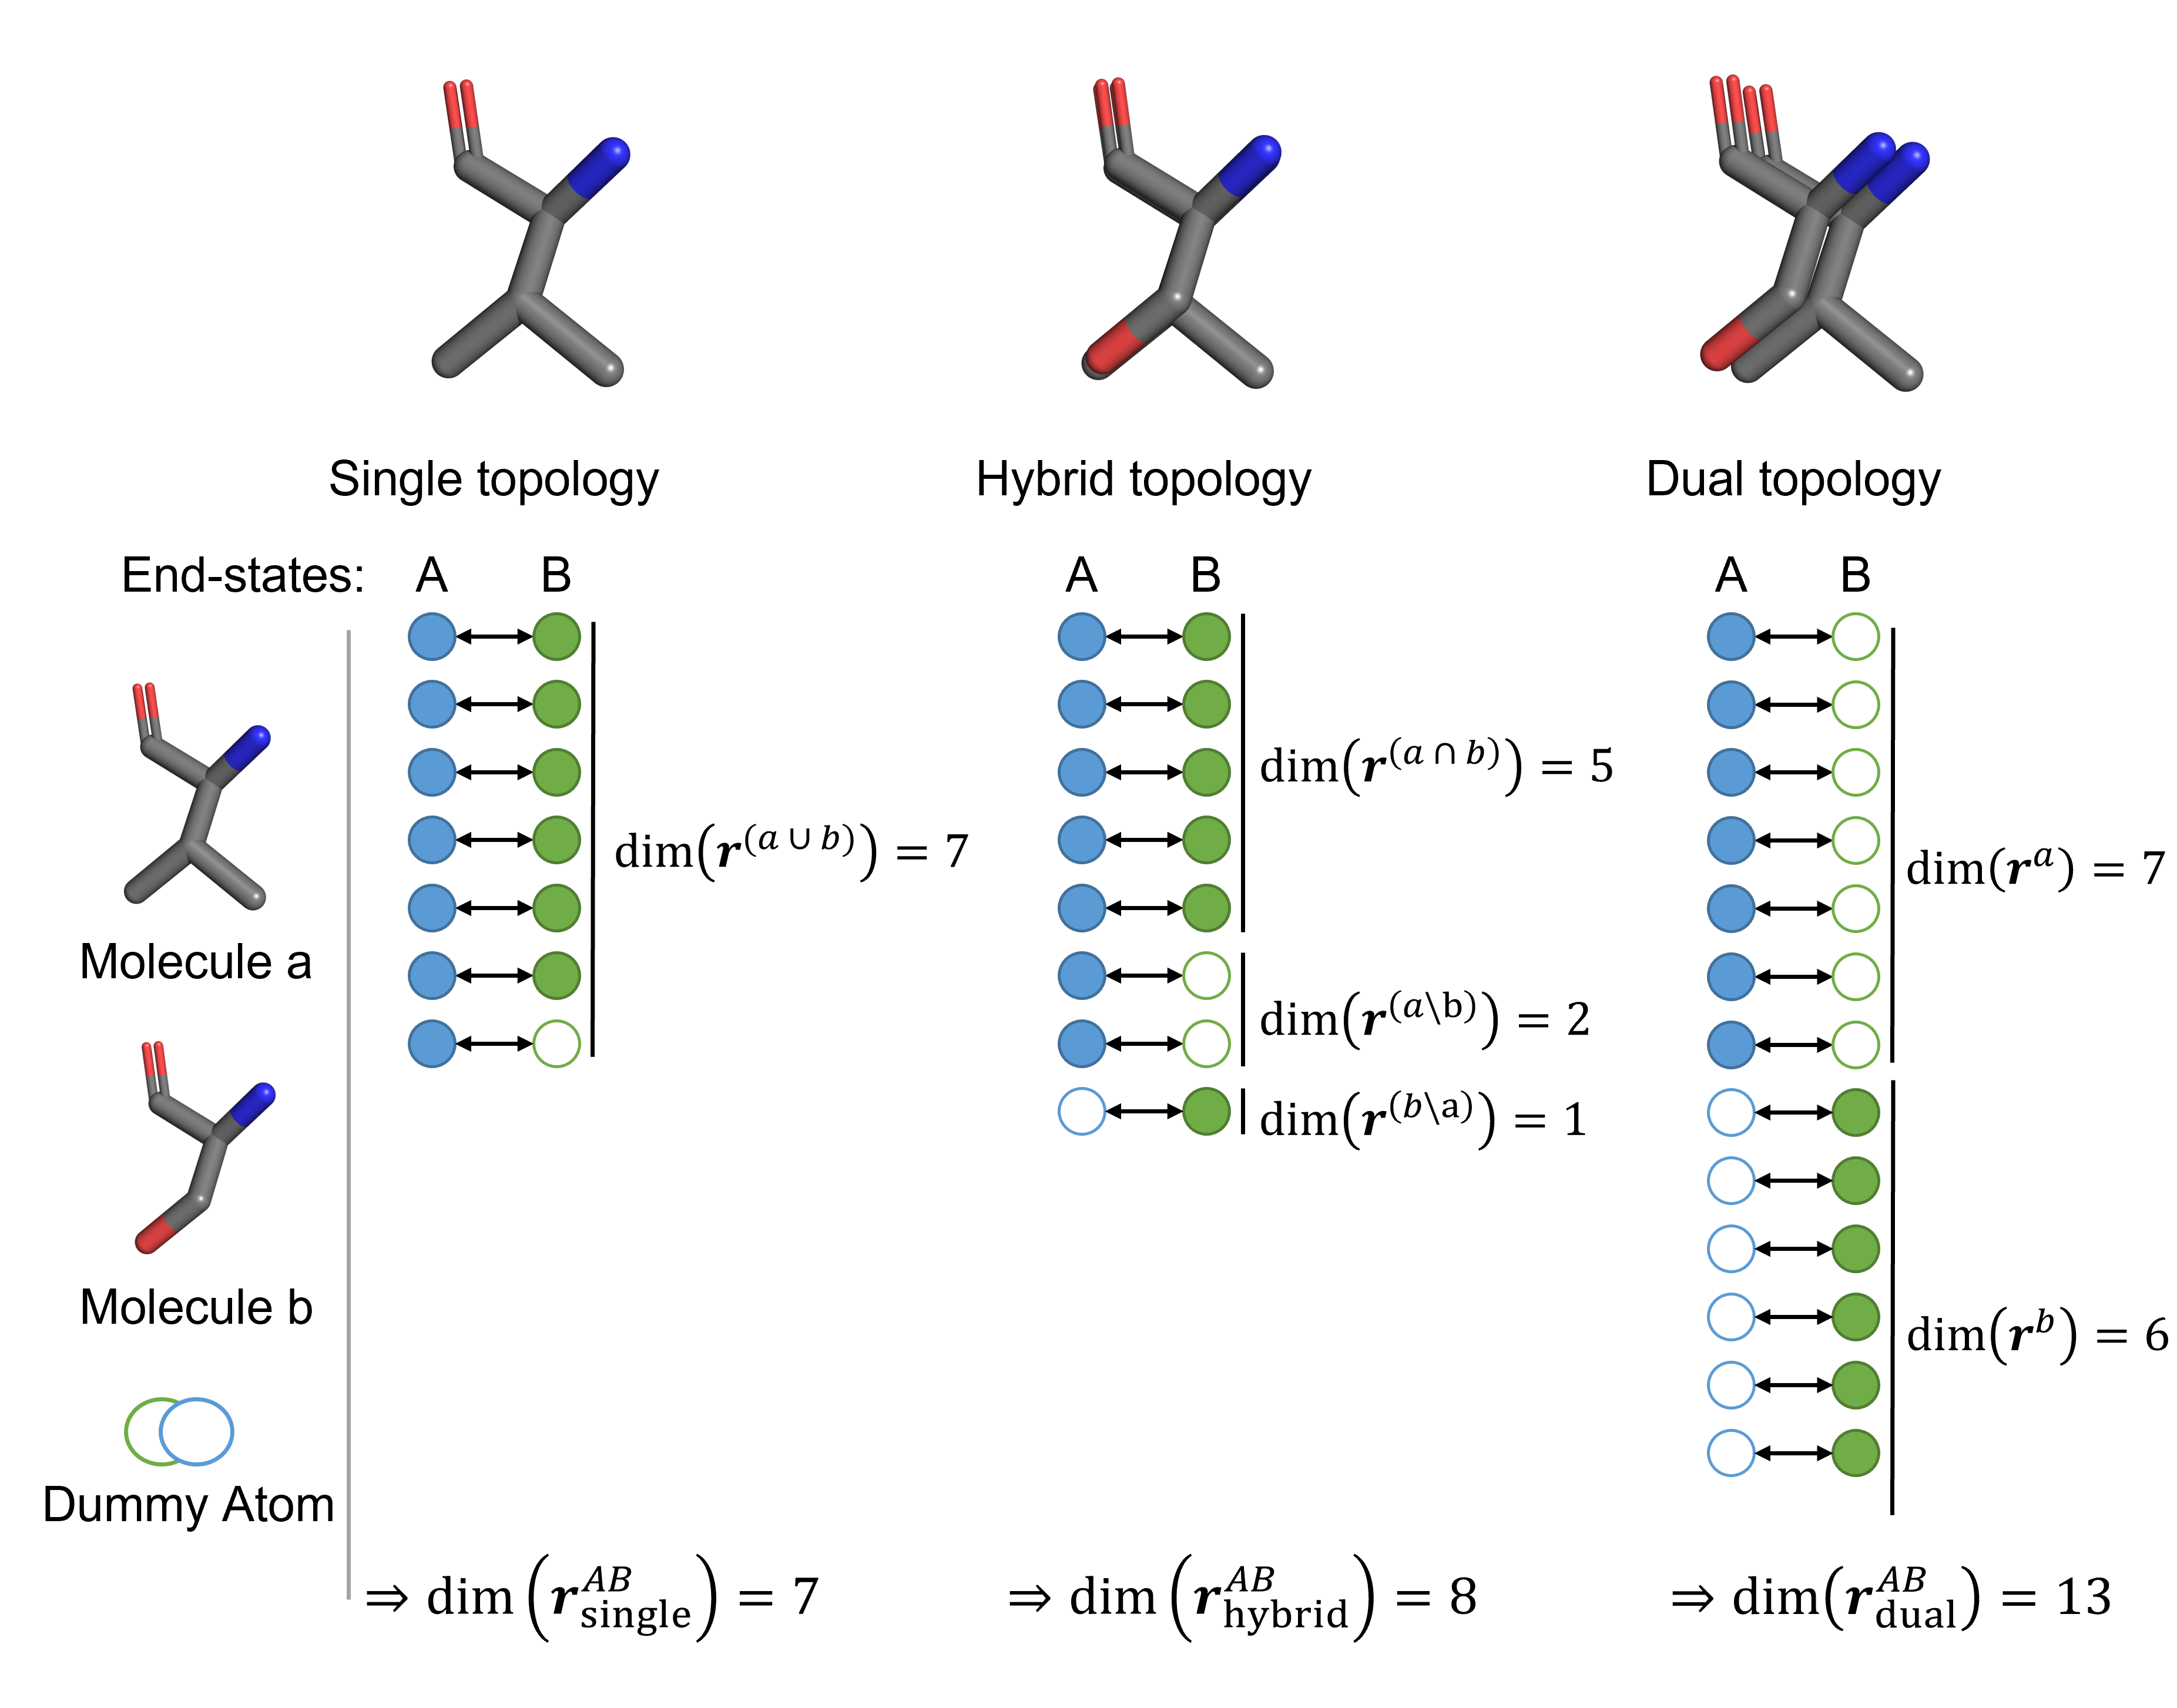
\includegraphics[width=\linewidth]{fig/theory/atomMappingSmallMols.png}
    \caption{The three end-state representations can be illustrated using the coordinate mapping of molecules $a$ and $b$ in the end-states $A$ and $B$, respectively. The smallest number of coordinates is required for the single topology coordinate space ($dim(\textbf{r}^{AB}_{\text{single}})$) as the coordinate set is formed from the union of all coordinates (left). If a coordinate is only used in one end-state, it becomes a non-interacting dummy atom in the other end-state. The hybrid topology approach (middle) requires more coordinates for its coordinate space ($\textbf{r}^{AB}_{\text{hybrid}}$), as the coordinates of differing atoms are represented separately. The largest coordinate space is required for the dual topology approach. Here, the coordinate space ($dim(\textbf{r}^{AB}_{\text{dual}})$) is the sum of both molecules.}
    \label{fig: AtomMapping}
\end{figure}

%%% single topology
\subsubsection{Single Topology}
%%%%Coordinate space
The single topology approach was first used by Jorgensen \textit{et al.}\cite{Jorgensen1985} to calculate the relative hydration free energies of methanol and ethane. The approach was later termed ``single topology'' by Pearlman \textit{et al.}.\cite{Pearlman1991}
The end-states are represented by the union of the coordinates of the molecules, limiting the possible transformations that can be handled by this method. Usually, perturbations for a single topology approach include both atom types (i.e. van der Waals parameters and/or partial charges) and bonded terms.\cite{Jorgensen1985, Pearlman1991, Pearlman1994, Boresch1999, Boresch1999B, Donnini2011, Donnini2016, Wang2015,  Liu2015, Wang2017, Damodaran2001}
%
A single topology approach in this definition is constructed as follows for two end-states $A$ and $B$ with the two molecules $a$ and $b$ (Figure \ref{fig: AtomMapping}),
\begin{align*}
dim(\textbf{r}_{single}^{AB}) &= dim(\textbf{r}^{(a~\cup~b)}) \\
    \textbf{r}^{AB}_{\text{single}} &= \{\textbf{r}^{~AB}_{1}, \textbf{r}^{~AB}_{2}, ..., \textbf{r}^{~AB}_{dim(\textbf{r}_{single}^{~AB})}\}\\
\end{align*}
where $dim(\textbf{r}_{single}^{AB})$ is the total number of atom coordinates of the end-states $A$ and $B$, and $\textbf{r}$ the coordinate space vector. Note that the unperturbed atoms of the environment (i.e., solvent and/or protein atoms), were excluded for simplicity.

%%%%Problems and solutions]
%%%%%%Sampling
The single topology approach has in principle the best sampling efficiency compared to other representations as it is constructed with the least amount of coordinates and therefore the fewest degrees of freedom are perturbed.\cite{Pearlman1994, Donnini2011, Yu2017, Fleck2021}
%%%%%Different Atoms
However, an issue arises when the molecules do not only differ in the type of atoms but also in their number. To address this, a non-interacting ``dummy'' state can be assigned to the vanishing atom(s).\cite{Pearlman1994, Donnini2011, Yu2017, Fleck2021}
Different variants of dummy states are possible. Typically, only the non-bonded interactions are removed. However, it has been shown that also the bonded terms of ``dummy'' states can influence the free-energy calculations.\cite{Fleck2021}
The construction of a single topology becomes increasingly challenging with more complex molecule transformations.
For example, to realize complex transformations such as ring size changes or ring opening/closing, special soft-bond terms had to be implemented.\cite{Wang2017} 

%%% hybrid topology
\subsubsection{Hybrid Topology}
The term hybrid single-dual topology was used by Jiang \textit{et al.}\cite{Jiang2019} in 2019 to describe the combination of a single-topology core (common among the molecules) with dual-topology substituents (differing among the molecules). However, similar schemes were already used in many previous studies (although called either single or dual topology).\cite{Eriksson1995,Shobana2000, Gapsys2015, Petrov2021, Seeliger2010, Riniker2011}
%Examples are the study by Shobana \textit{et al.}\cite{Shobana2000} for amino acid mutations, or the study by Eriksson \textit{et al.}\cite{Eriksson1995} for a base pair exchange in DNA. 
%
A hybrid topology approach in this definition can be constructed as follows for two end-states $A$ and $B$ with the two molecules $a$ and $b$ (Figure \ref{fig: AtomMapping}),
\begin{align*}
    dim(\textbf{r}_{hybrid}^{AB}) &= dim(\textbf{r}^{~(a~\cap~b)}) + dim(\textbf{r}^{~(a \setminus b)}) + dim(\textbf{r}^{~(b \setminus a)})\\
    \textbf{r}^{AB}_{\text{hybrid}} &= \{\textbf{r}^{~(a~\cap~b)}_{1}, \textbf{r}^{~(a~\cap~b)}_{2}, ..., \textbf{r}^{~(a~\cap~b)}_{dim(\textbf{r}^{~(a~\cap~b)})}, \\
    &~~~\textbf{r}^{~(a \setminus b)}_{1}, \textbf{r}^{~(a \setminus b)}_{2}, ..., \textbf{r}^{~(a \setminus b)}_{dim(\textbf{r}^{~(a \setminus b)})}, \\
    &~~~\textbf{r}^{~(b \setminus a)}_{1}, \textbf{r}^{~(b \setminus a)}_{2}, ..., \textbf{r}^{~(b \setminus a)}_{dim(\textbf{r}^{~(b \setminus a)})}, \}
\end{align*}
 
%%%%%%
Hybrid topology approaches aim a combining the advantages of single and dual topology, i.e., to keep the number of perturbed degrees of freedom minimal for sampling efficiency while facilitating more complex transformations.

%%%Dual Topology
\subsubsection{Dual Topology}
In a dual topology, two fully separate sets of coordinates are used for the molecules. This approach was first introduced by Gao \textit{et al.},\cite{Gao1989} and termed later on ``dual topology'' by Pearlman \textit{et al.}\cite{Pearlman1991} The atoms of molecule $a$, which are fully interacting in end-state $A$, are transformed to the dummy state in end-state $B$, and vice versa. Importantly, the atoms of the molecules do not interact with each other and only share the same environment.\cite{Riniker2011, Rocklin2013} In such dual topology approaches usually only the non-bonded terms are perturbed.\cite{Riniker2011, Sidler2016, Boresch1999, Michel2010}
%
A dual topology approach in this definition can be constructed as follows for the end-states $A$ and $B$ with the two molecules $a$ and $b$ (Figure \ref{fig: AtomMapping}),
\begin{align*}
    dim(\textbf{r}_{\text{dual}}^{~AB}) &= dim(\textbf{r}^{~a}) + dim(\textbf{r}^{~b})\\
    \textbf{r}^{AB}_{\text{dual}} &= \{\textbf{r}^{~a}_{1}, \textbf{r}^{~a}_{2}, ..., \textbf{r}^{~a}_{dim(\textbf{r}^{~a})}, \textbf{r}^{~b}_{1}, \textbf{r}^{~b}_{2}, ..., \textbf{r}^{~b}_{dim(\textbf{r}^{~b})}\}\\
\end{align*}

%%%% Sampling
The separated coordinates lead to a larger number of atoms in the system and thus, more degrees of freedom are perturbed, lowering the sampling efficiency compared to single topology approaches. 
Three sub-variants of the dual topology approach can be distinguished depending on how this issue is addressed in practice:
(i) the linked variant with direct spatial restraints between the molecules to prevent them from drifting apart during the simulation,\cite{Riniker2011, Sidler2016, Christ2009A, Jespers2019} (ii) the separated variant with restraining to the environment,\cite{Mobley2006, Rocklin2013} and (iii) the unconstrained variant.\cite{Henine2004, Carvalho2021}
The linked dual topology is in principle the most efficient variant if the transformation is relatively simple (no changes in binding modes induced by reorientation or large conformational differences). The separated dual topology approach is expected to be less efficient than the linked variant, but can handle these very challenging transformations.\cite{Mobley2006}
%%%% Transformation
A significant advantage of the dual topology approach is the straightforward set-up of a system compared to the single and hybrid topologies, especially for more complex transformations or multiple end-states.

\subsection{Automated Placement of Distance Restraints}
To facilitate the set-up of RBFE calculations with the linked dual topology approach, the selection of optimal distance restraints between the molecules needs to be automated.
The proposed algorithm is based on classical graph algorithms. Its goal is to identify suitable placements for the distance restraints between two molecules $m_i$ and $m_j$.
%
The following conditions are applied:
\begin{enumerate}
    \item $m_i$ and $m_j$ are pre-aligned to each other 
    \item Optimal placement of distance restraints requires that 
    \begin{enumerate}
        \item the restrained atom pairs are maximally distant over the two molecules
        \item the restrained atoms have a small distance to each other in the aligned structures
        \item the restraints do not influence the conformational sampling of the molecules
    \end{enumerate}
    \item For a user-defined number of required restraints $n_{\text{res}}$, it holds that $n_{\text{res}} \ll n_{m_i} $ and $ ~n_{res} \ll n_{m_j}$ , where $n_i$ and $n_j$ are the numbers of atoms of molecules $m_i$ and $m_j$, respectively
\end{enumerate}
From these conditions follows that only atoms in relatively rigid regions of the molecules such as rings should be selected for the restraint search space. While restraining non-ring atoms might be favorable for the maximally distant distribution of the restrained atoms over the molecules, it is more likely to distort the conformational sampling of the molecules. The steps of the algorithm are shown schematically in Figure \ref{fig:algorithmScheme} and explained in the following subsections.

\subsubsection{Assigning Distance Restraints for a Pair of Molecules}
\begin{figure}[h!]
    \centering
    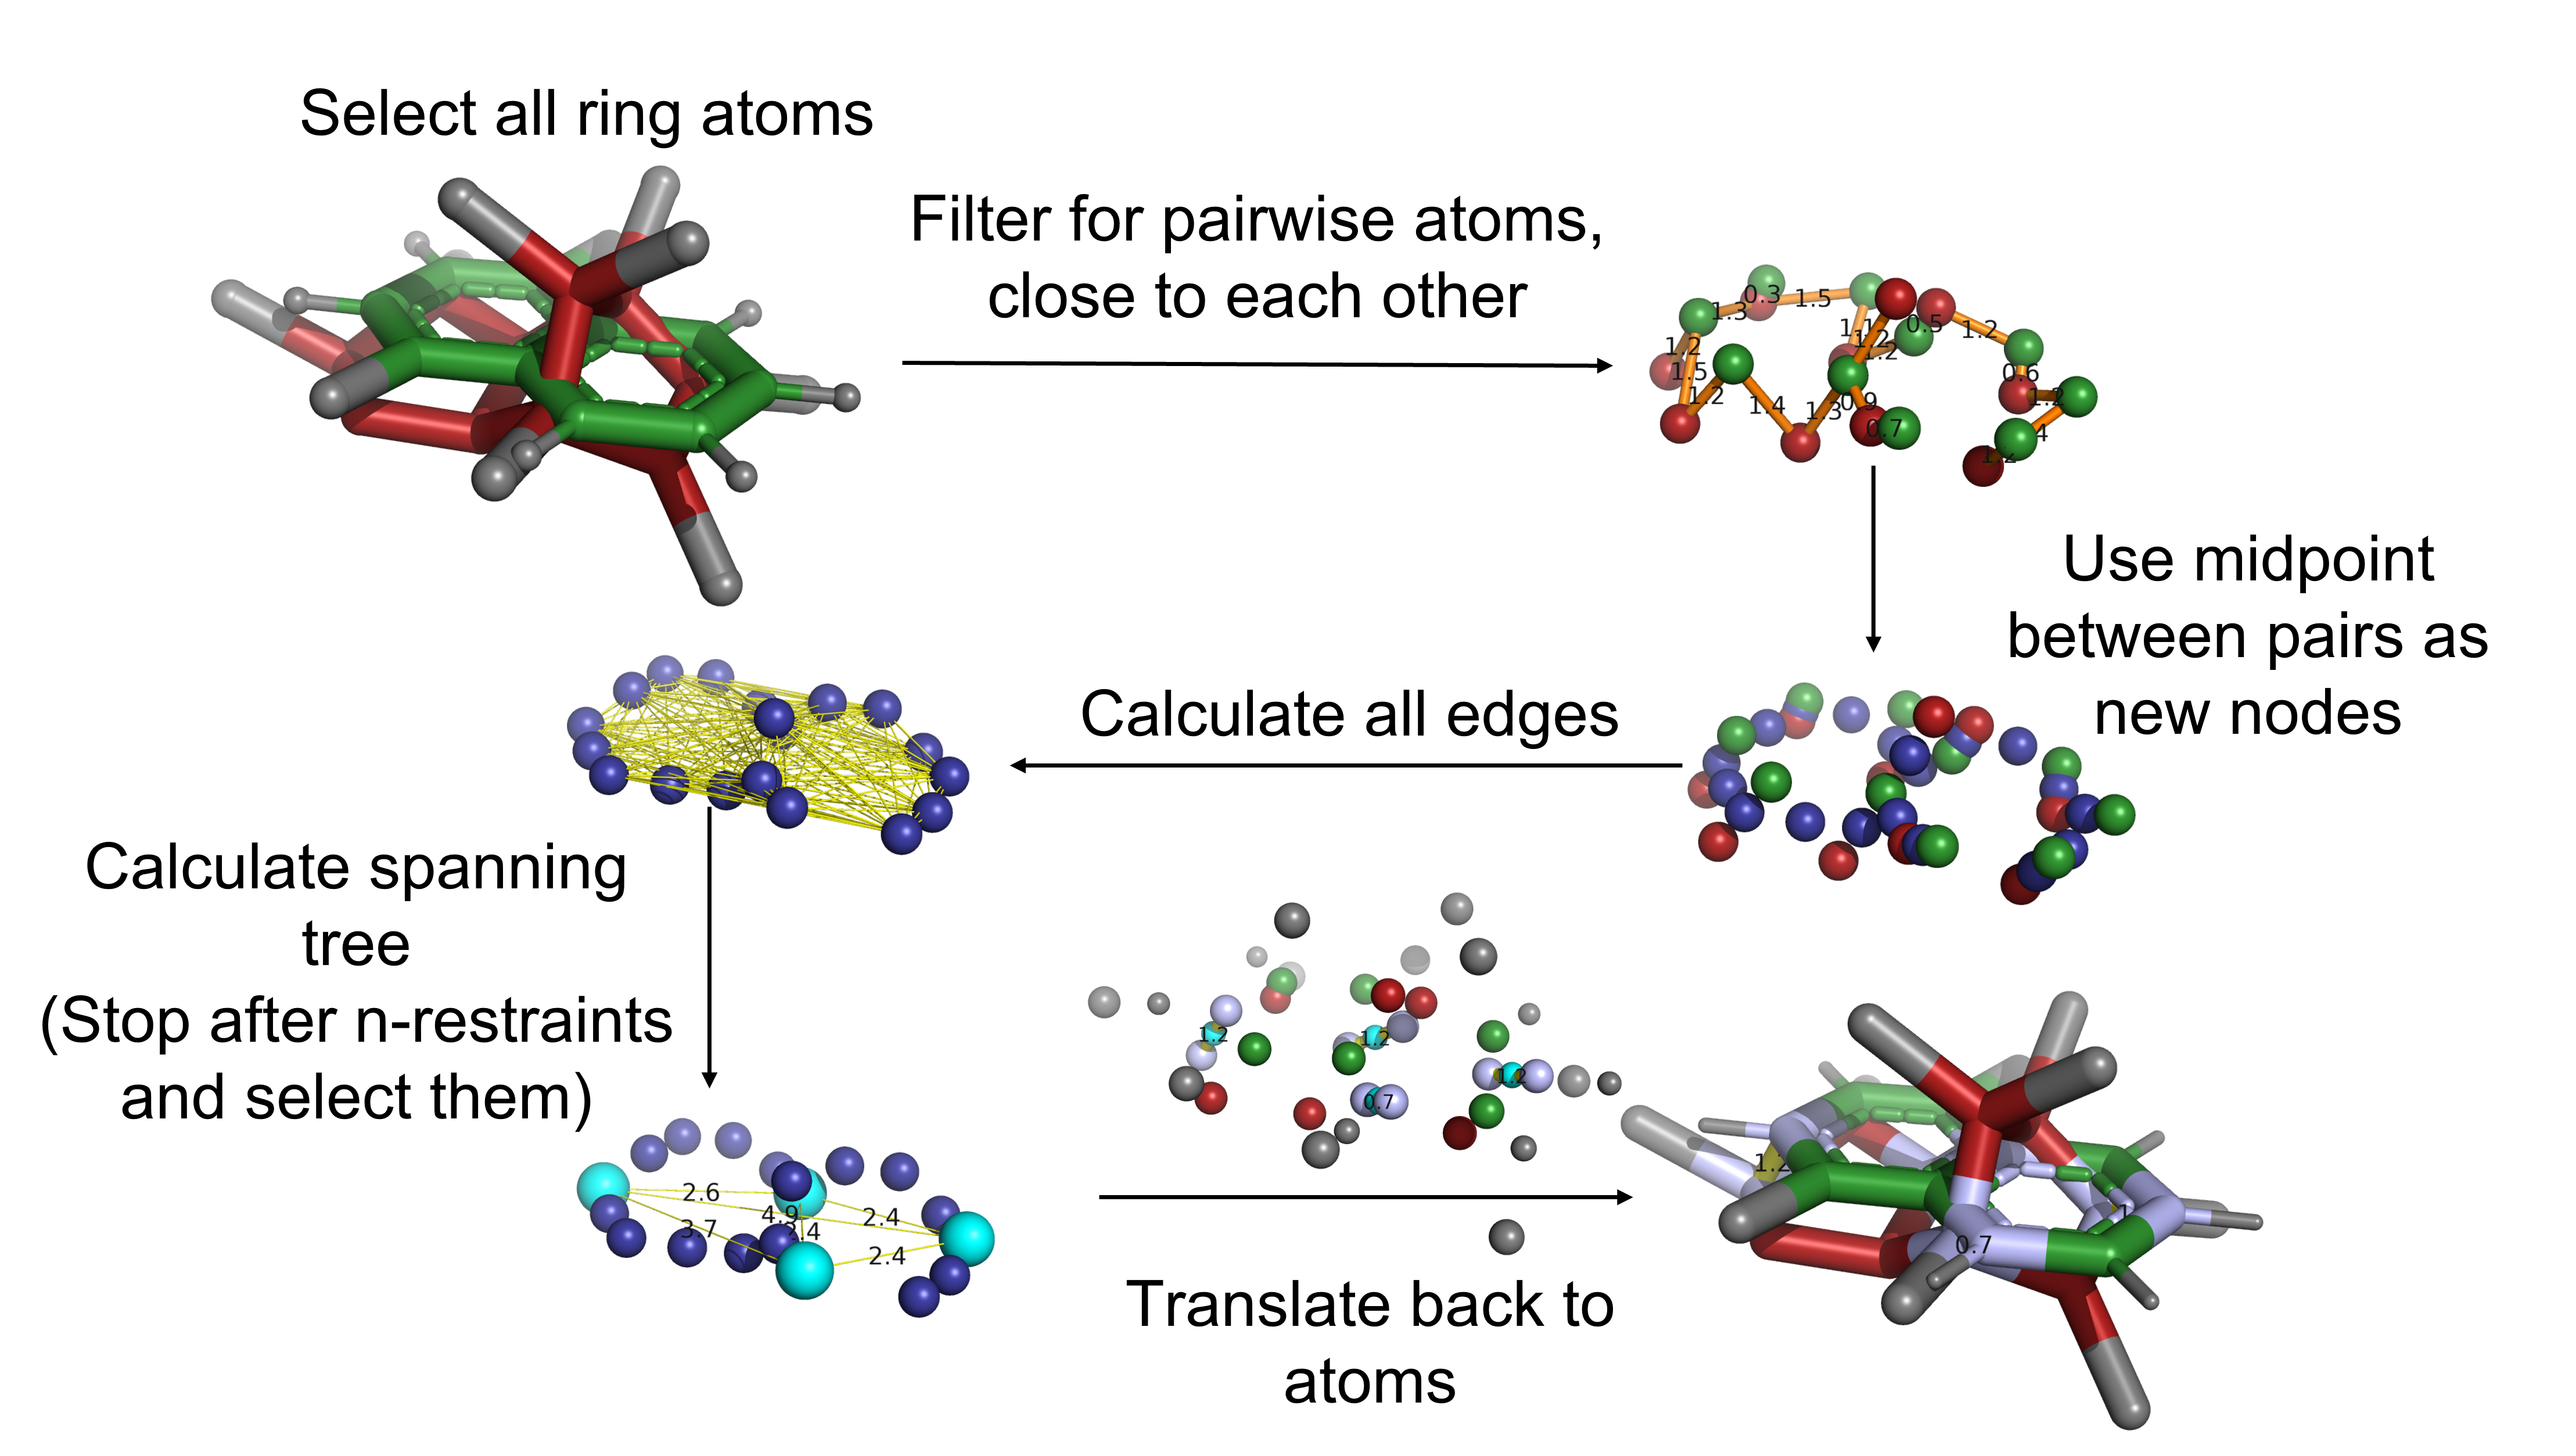
\includegraphics[width=\textwidth]{fig/theory/AlgorithmScheme.png}
    \caption{Schematic illustration of the algorithm steps to identify optimal placements for the distance restraints between a pair of molecules. The described algorithm uses a set of possible atoms (here these are the ring atoms). Next, possible restraints are filtered by the user-defined atom distance cutoff $d_\text{res}$. After this filtering step, the midpoints of the remaining possible restraints are calculated and used further as nodes of a graph. These nodes are connected by edges that have assigned weights, corresponding to the Euclidean distance of the midpoints. From this, a spanning tree is built with a min-max decision scheme. The construction of the spanning tree is stopped after $n_\text{res}$ iterations or if all nodes were connected. The result is a set of optimal restraints, $C_{\text{res,opt}}$, which will be translated back to an atom selection for further use in MD packages.}
    \label{fig:algorithmScheme}
\end{figure}

\noindent\textit{Translation into a graph problem}:
The developed algorithm is based on a graph representation of the restraint search space. To solve the problem of selecting an optimal set of atom pairs to define the distance restraints, it needs to be translated into a graph $G$ fulfilling,
\begin{equation}
    G(N, E, \omega), E \subseteq \{\{x,y\}\mid x,y\in N\;{\textrm {and}}\;x\neq y\},
\end{equation}
where $N$ is a set of nodes, $E$ a set of edges, and $\omega$ a set of weights.

We consider a molecule pair consisting of the two molecules $m_i$ and $m_j$, with their sets of atoms $A_i$ and $A_j$, respectively. 
%%Alignment
In a first step, existing algorithms such as e.g. implemented in the RDKit\cite{Landrum2021} or PyMol\cite{Delano2020} can be used to align the two molecules to each. The alignment can for example be based on the maximum common substructure (MCS), or in the case of scaffold hopping the maximal overlap of the van der Waals volumes of the molecules.
%%Filter
Next, the sets of possible atoms $A_i$ and $A_j$ for the distance restraints are reduced to the ring atoms of the respective molecules, $A^\text{ring}_i$ and $A^\text{ring}_j$. 
%% Restraints with a Distance cutoff
In addition, a user-defined cutoff distance $d_\text{res}$ between the atom pairs is introduced (here, $d_\text{res} = 0.1~\text{nm}$). 
Therefore, a possible distance restraint is a pair of atoms $(a^\text{ring}_i, a^\text{ring}_j)$ that fulfills the distance criterion $d(a^\text{ring}_i, a^\text{ring}_j) \leq d_\text{res}$.

%% Building a Graph
The possible distance restraints $C_\text{res}$ are used as nodes $N$ to construct a fully connected graph $G$. 
Each individual restraint $c_\text{res}$ is represented by the midpoint of the two involved atoms.
The undirected edges of $G$ have as weight $\omega^\text{dist}_{ji}$ the Euclidean distance between the midpoints of the two atom pairs $\omega^{dist}_{ji}=d(c_{\text{res}_j},c_{\text{res}_i})$. \\

\noindent\textit{Solving the graph problem}:
From the generated graph, only a subset of restraints fulfills the conditions 1-3 listed above.To obtain a relevant subset of restraints, we decided to use a min-max decision scheme inspired by the minimax theorem \cite{Neumann1928} to build a spanning tree (i.e. a subset of restraints, $C_\text{res,opt}$) within a greedy Prim-like approach.\cite{Prim1957}

%Algorithm Definition
%%bit more literature research
%initial move
The algorithm starts by picking the edge in the graph $G$ with the largest weight $\omega^\text{dist}_{ij}$ (distance), i.e. the two restraints whose midpoints are the furthest apart. 
%iterate
%%update min
After this initial selection of two restraints for $C_\text{res,opt}$, the weights of the edges in $G$ are updated with the minimal distance of all $c_\text{res}$ in $C_\text{res,opt}$ to a respective node $n_i$. Subsequently, all edges and nodes are removed, which contain atoms that are already selected in $C_\text{res,opt}$.
%% select max
After the update of the edge weights, the restraint $c_\text{res}$ with maximal $\omega^\text{dist}_{ji}$ is added to $C_\text{res,opt}$.
%%termination
This procedure is repeated until either $|C_\text{res,opt}| = n_\text{res}$ (in practice we expect a rather small number for $n_\text{res}$, typically $ 4 < n_\text{res} < 10$) or all remaining nodes are connected. \\

\noindent \textit{Back-mapping}:
The selected subset of $n_\text{res}$ restraints, $C_\text{res,opt}$ is mapped back to the atoms in the molecules, such that the distance restraints can be written in a format readable by MD packages such as GROMOS\cite{Schmid2012} or GROMACS.\cite{Abraham2015} Additionally, a JSON\cite{Pezoa2016} format is provided, allowing to import the results with any standardized JSON-Parser. \\

\noindent \textit{Tie-breaking}:
Due to non-perfect alignment and finite numerical precision, a tie between multiple restraints can occur, i.e. they have a very similar distance to the already selected restraints. This practical problem was solved by adding a tie-breaker that detects whether multiple high-priority restraints are within a range of $0.02$~nm in a given iteration step and refines the decision result by applying a second criterion. 
For each candidate restraint in an iteration step, the distance to the center of geometry (COG) of all already selected restraints is calculated, and the restraint is chosen for which this distance is maximal.


\subsubsection{Extension to Multiple End-states}

For multi-state methods such as EDS\cite{Christ2007,Christ2008}, replica-exchange EDS (RE-EDS)\cite{Sidler2016,Sidler2017,Ries2021B}, multi-site $\lambda$-Dynamics,\cite{Knight2011} or multi-state $\lambda$-LEUS,\cite{Bieler2015} more than two molecules need to be restrained to each other. Based on our experience with RE-EDS, it is best to apply the distance restraints between multiple molecules in form of a ring, i.e. each molecule is restrained to two neighboring molecules.\cite{Ries2021B} This scheme is used in the following.

\begin{figure}[h!]
    \centering
    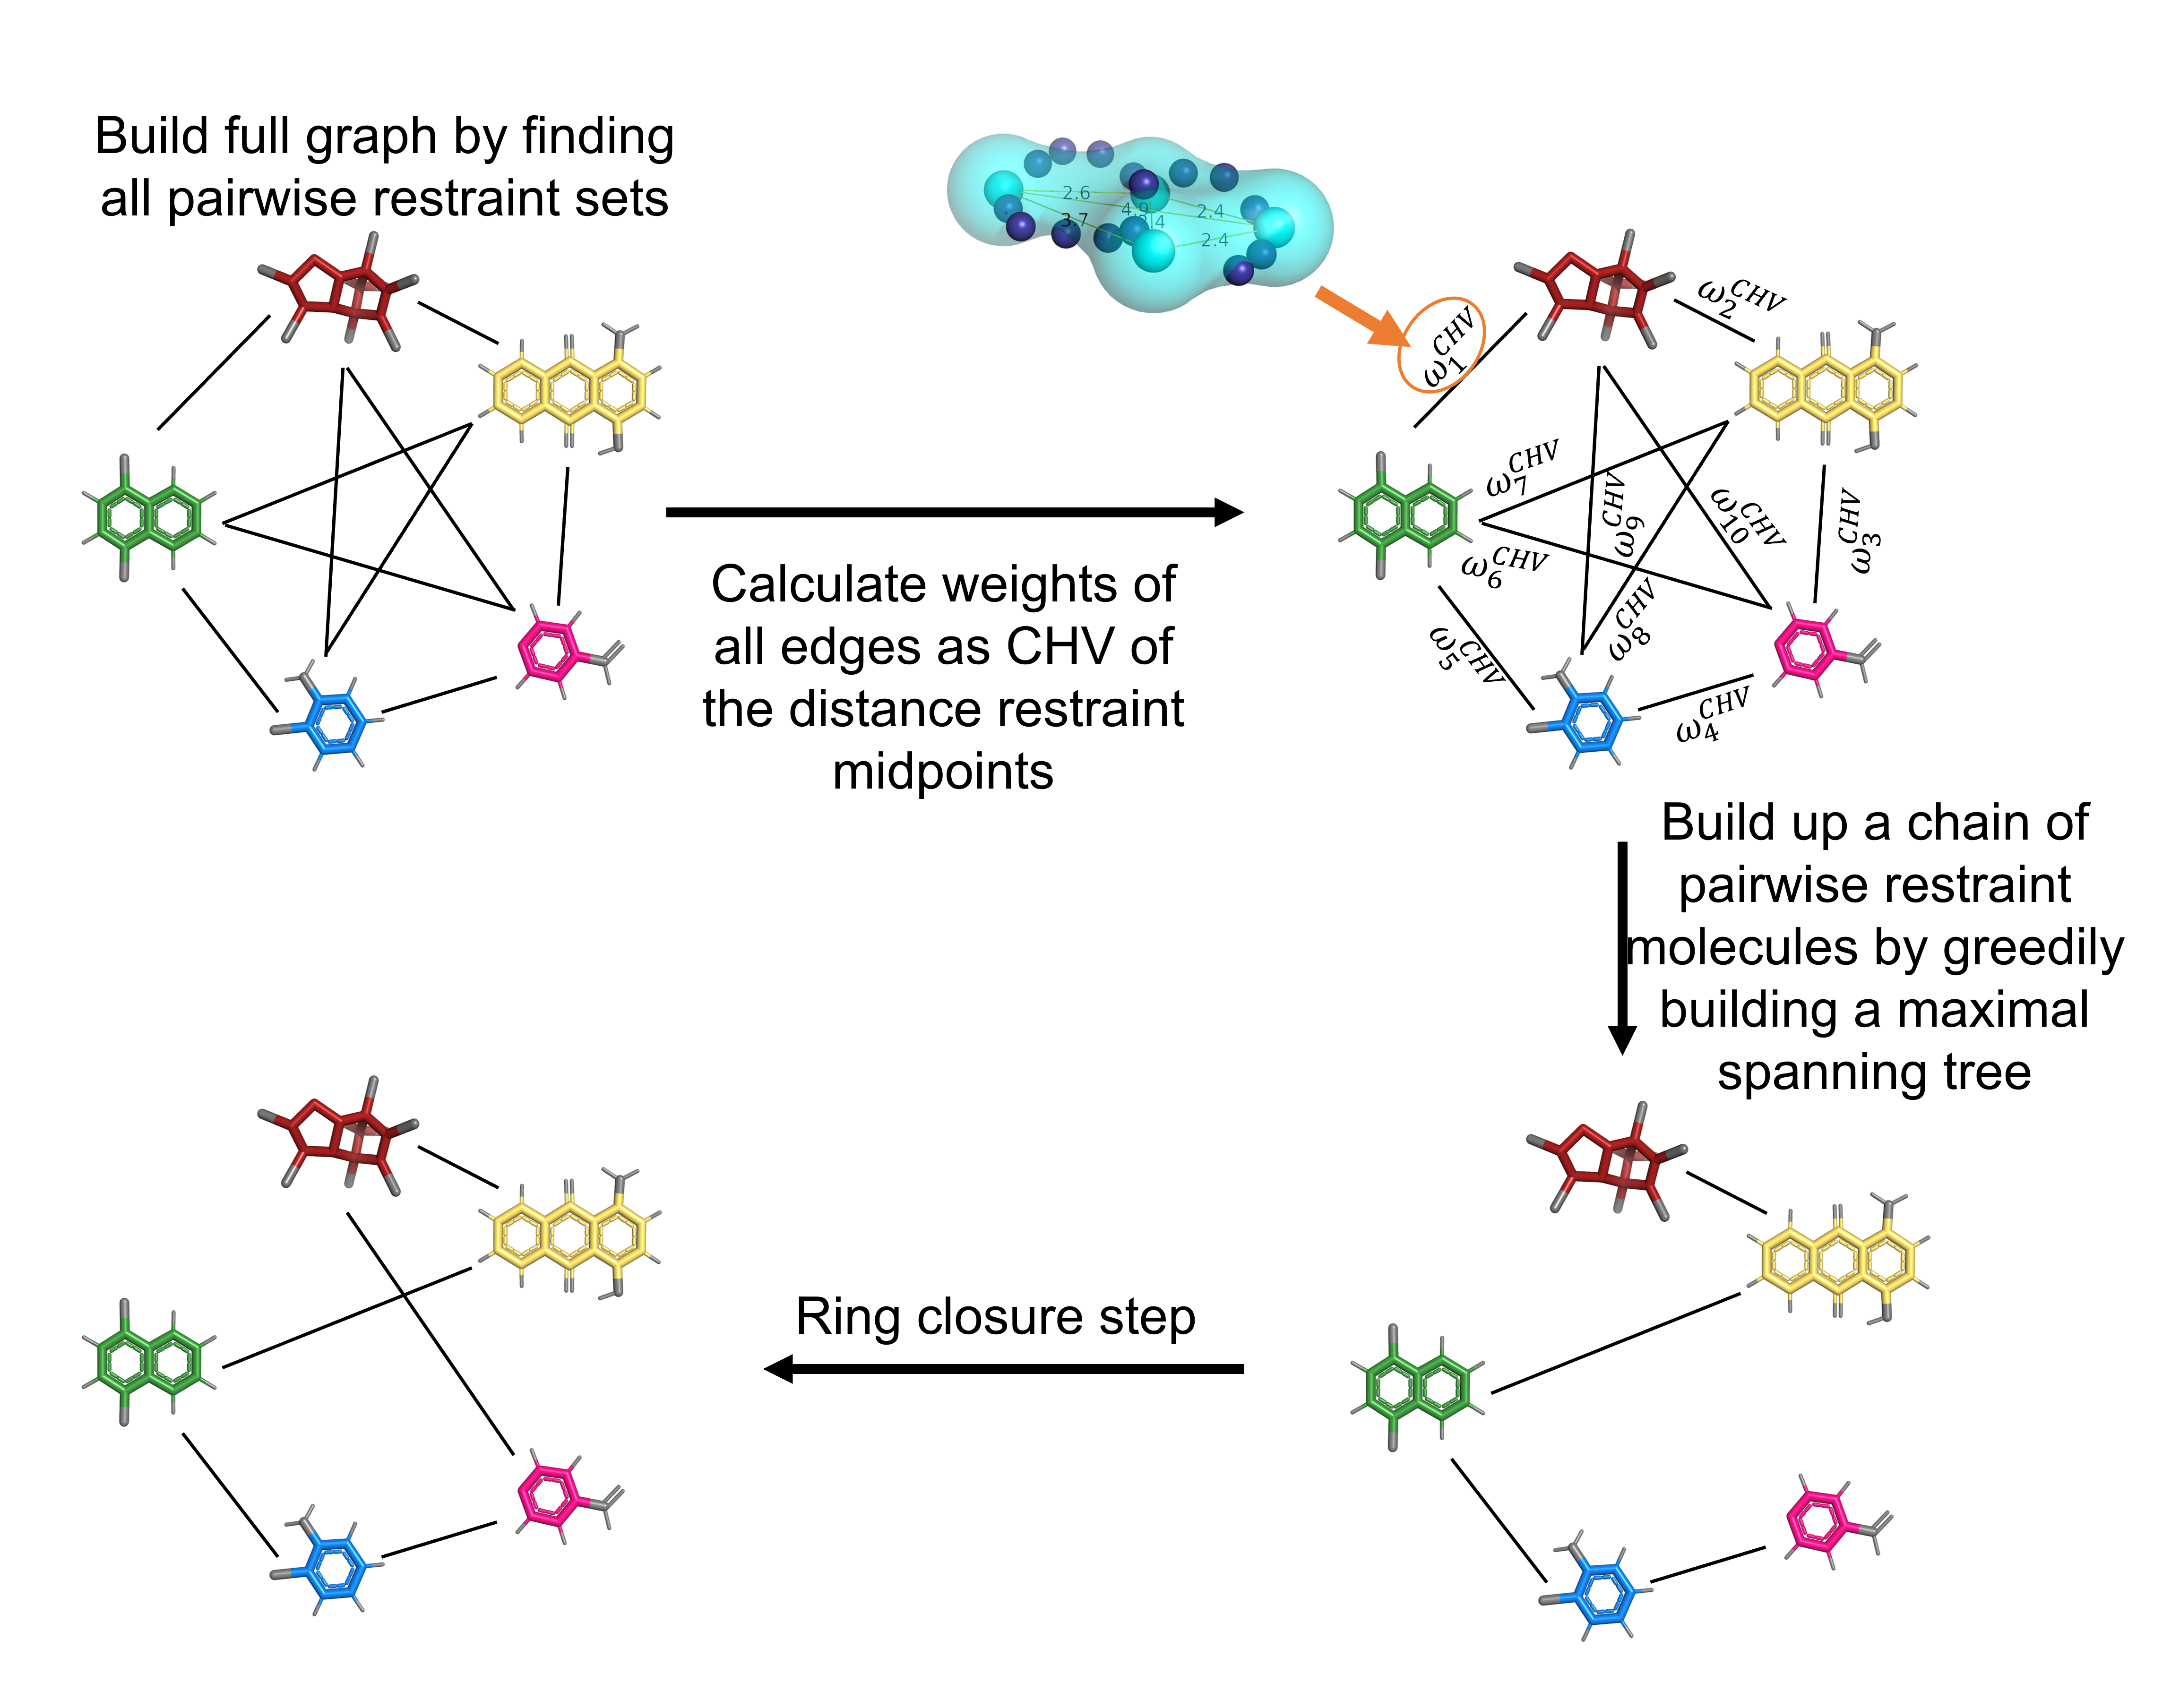
\includegraphics[width=\textwidth]{fig/theory/MultistateExpansion.png}
    \caption{Schematic illustration of the algorithm steps to link multiple end-states by distance restraints for a multi-state RBFE calculation. The selection is carried out in four steps. (i) Optimal restraints are calculated for all possible molecule pairs, building up a fully connected graph. (ii) The weights $\omega^\text{CHV}_i$ of the edges are calculated as the convex hull volume (CHV) formed by the selected restraints. (iii) A maximum spanning tree without branching is greedily constructed by selecting the edges with maximal weights. (iv) The ring is closed by connecting the ends of the chain.}
    \label{fig: convexHull}
\end{figure}

In a first step, the pairwise greedy algorithm is used to calculate an optimal set of distance restraints between all possible molecule pairs, building up a fully connected graph (Figure \ref{fig: convexHull}). The possible sets of restraints are subsequently compared to each other by calculating the convex hull around the coordinates of all the restraint midpoints. The convex hull volume (CHV) is then assigned to the edges of the fully connected graph as weight $\omega^\text{CHV}$. The optimal chain of connected molecules is determined by applying another greedy algorithm, inspired by the Kruskal algorithm,\cite{Kruskal1956} which picks the edges with the largest CHVs without forming cycles or branches (Figure \ref{fig: convexHull}). The chain is closed to a ring by tying the loose ends together. This last molecule pair may have a less good set of restraints.

\FloatBarrier

\subsection{Free-Energy Methods}
Two free-energy methods were tested with the linked dual topology approach.

\subsubsection{Thermodynamic Integration}
TI is a standard method to estimate free-energy differences,\cite{Kirkwood1935} where a $\lambda$-dependent path between the two end-states $A$ and $B$ is sampled. The potential energy of the system is constructed as,
\begin{equation}
    V(\textbf{r}; \lambda) = (1-\lambda) ~ V_A(\textbf{r}) + \lambda ~ V_B(\textbf{r})
    \label{eq: TI-Potential}
\end{equation}
End-state $A$ is obtained when $\lambda = 0$, and end-state $B$ when $\lambda = 1$. In practice, simulations at discrete $\lambda$-points between 0 and 1 are performed, and the free-energy difference is obtained by numerical integration,
\begin{equation}
    \Delta G^{rel}_{BA} = \int^{1}_{0} \left< \frac{\partial V(\lambda)}{\partial \lambda} \right>_{\lambda} \,d\lambda
    \label{eq: TI-Integration}
\end{equation}

\subsubsection{Replica-Exchange Enveloping Distribution Sampling}
%% Hamiltonian Construction
RE-EDS\cite{Sidler2016,Sidler2017,Ries2021B} is a combination of Hamiltonian replica exchange\cite{Hansmann1997,Sugita2000} and EDS.\cite{Christ2007,Christ2008} In EDS, a reference state Hamiltonian $V_R$ is sampled, which combines $N$ end-states as,
\begin{align}
    V_R\left(\textbf{r};s,\textbf{E}^R\right) = -\frac{1}{\beta s}\ln\left[\sum\limits_{i=1}^N e^{-\beta s\left(V_i(\textbf{r})-E_i^R\right)}\right]
\end{align}
where $s$ is the smoothness parameter, $E_i^R$ a set of energy offsets and $\beta=1/(k_B~T)$, where $k_B$ is the Boltzmann constant and $T$ the absolute temperature. 
The force on a particle $k$ can be calculated as, \cite{Christ2007,Christ2008}
\begin{align}
    \textbf{f}_k(t)=-\frac{\partial V_R(\textbf{r}; s, \textbf{E}^R)}{\partial \textbf{r}_k} = \sum^N_{i=1}\frac{e^{-\beta s(V_i(\textbf{r}) -E_i^R)}}{\sum^N_{j=1}{e^{-\beta s (V_j(\textbf{r})-E_j^R)}}}  \left( -\frac{\partial V_i(\textbf{r})}{\partial \textbf{r}_k} \right) \,.
\end{align}
For high $s$-values (close to 1.0), the sampling of the reference state is dominated by the end-state with the lowest value of $V_i(\textbf{r}) - E_i^R$, whereas for small $s$ values (close to zero), all end-states contribute to the forces, resulting in the so-called ``undersampling''.\cite{Riniker2011} 

The free-energy difference between a pair of end-states in the system is then calculated as,
\begin{align}
    \Delta G^{rel}_{BA} = -\frac{1}{\beta}\ln\frac{\langle e^{-\beta(V_B-V_R)}\rangle_R}{\langle e^{-\beta(V_A-V_R}\rangle_R} \, .
\end{align}
In practice, an optimal choice of $s$ and $E_i^R$ is essential to sufficiently sample all end-states in an EDS simulation. RE-EDS overcomes the difficulty of choosing an optimal $s$-value by simulating multiple replicas with different $s$-values and performing replica exchanges between them.\cite{Sidler2016,Sidler2017}
